%change inverted comma of “bad” in P3, 3x punctuation , in P5; title in P6 
%Added index to Granny Dot’s
\chapter{You are your thoughts}
\addcontentsline{toc}{chapterdescription}{Your thought forms come first, lenses you see actuality through, before your meaning-making stories even generate your experienced reality. Once you have mastered binary logical thinking you have the foundations for the 28 post-logical thought forms, or lenses, of the next stage: Process, Context, Relationship and Transformation thought forms. The more fluidity you have in these, the better you grasp actuality and can make your reality a good model of it.}
%\addcontentsline{toc}{chapterdescription}{\pagebreak}
\label{chapter:who-am-i-sense}


\begin{chapterquotation}
I paint objects as I think them, not as I see them. \\
\raggedleft\textemdash Pablo Picasso\index{Picasso, Pablo}
\end{chapterquotation}




Before you can make meaning of anything that happens, you need to assemble an image, an inner representation of it, in your thoughts. 


The more fluidity you have in using a wide range of different forms of thought, i.e., lenses, the better that this image will be in making you aware of what is important for you, and hide what is not. The better that your thoughts can do this, the more useful and realistic will be the meaning that your stories can make of it.


In this section I will describe the difference between how we think and what we think. You will also finally learn the 28 different forms\index{thought forms (28)} of thought, or post-logical lenses, that we have mentioned numerous times so far in this book, the forms of thought going beyond simple opposites to complementary pairs; and that you can only begin to develop after you have mastered binary logic.


\begin{quote} 
Contraria Sunt Complementa\textemdash \emph{Opposites are complementary}
\end{quote} 


is the motto the quantum physics pioneer Niels Bohr\index{Bohr, Neils} chose for his coat of arms when granted the Danish Order of the Elephant in 1947. 


By the time most of us have finished our formal education, we have become very good at using logical forms of thought. We know that the opposite of right is wrong. We know that the opposite of true is false. We know that something is either right or wrong, true or false. Never right and wrong, true and false.


Binary logic forms of thought only work if your world is simple, or at most complicated\footnote{The Cynefin framework in the list on Page~\pageref{list:cynefin} is a very useful way of deciding if your challenge is obvious/simple, complicated, complex, chaotic or disordered\cite{snowden-cynefin, cynefin}.}. As soon as your world is nebulous, volatile, uncertain, complex or ambiguous, you need to go beyond binary logic.\index{binary logic}


As Figure~\ref{figure:truth-square} shows, the opposite of \emph{true} may simply be \emph{a different truth}. The opposite of a deep truth may well be an equally deep truth, not a falsehood. To make sense of your world and options, you may need to hold both deep truths in your head simultaneously, even though they visibly contradict each other.


\begin{SCfigure}[0.7][htb]
%\begin{wrapfigure}{O}{0.55\textwidth}
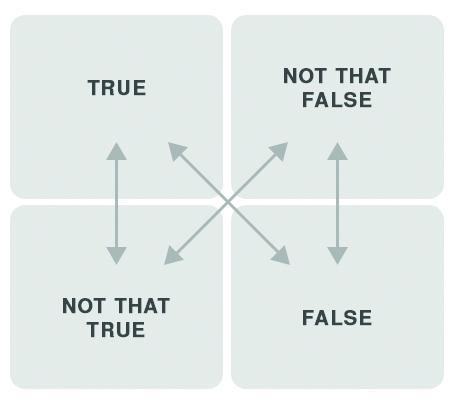
\includegraphics[width=0.45\textwidth]{./Images/truth-square}
\caption{Truth square. The opposite of true is not always false.}
\label{figure:truth-square}
%\end{wrapfigure}
\end{SCfigure}


The 28 post-logical forms of thought\index{thought forms (28)} are all those necessary to be able to simultaneously hold all the realities needed to make sense of the biggest adaptive challenges you will ever face in your life. Then you will have the most powerful capacity for sense-making anyone can have, enabling you to rise to any adaptive challenge.


We have two kinds of thinking, and these thought forms as well as binary logic can be in both. One, called Type~1, costs us very little effort. Only the thought forms we are extremely fluid in show up in Type~1. Type~2 is much slower and costs us far more effort because we are thinking deliberately. Here we can also apply forms and content of thought that we are still learning to use. 


These two types of thinking are described in detail in the excellent book \emph{Thinking Fast and Slow}\index{Thinking Fast and Slow} by Daniel Kahneman\cite{kahneman-thinking}.\index{Kahneman, Daniel} In Type~1 thinking, your thought forms are on autopilot and activate a narrow set of well-used stories. Perfect if you're facing a challenge that you have faced many times before and have the skills you need to rise to the challenge. But a disaster if you only use Type~1 thinking to respond to a VUCA\index{VUCA} challenge that you have never seen before.


The more any part of your life, but especially your work, involves change, contradiction, or wholes that must be completely included, the more you can only succeed with a sufficiently high fluidity in the 28 forms of post-logical thinking\index{thought forms (28)} in Table~\ref{table:28DTF}. I sometimes call all 28, transformational thinking, even though only the final seven strictly qualify as transformational thinking\footnote{Otto Laske, pioneer of using these thought forms practically in business, these are called dialectic thought forms. I have mostly avoided using the word dialectic\index{dialectics} in a book about economics to avoid adding in any interpretations you associate with Marx's dialectics. \index{Marx, Karl} These thought forms are pure forms, and have nothing to do with the content or meaning of Marxist dialectics. Of course, Marx used these forms himself.}.


A recent example of transformational thinking from me (Graham). There have been times when I have felt all-powerful, capable of doing everything, over the past years starting up Evolutesix.\index{Evolutesix} And there have been times when I have felt weak, overwhelmed by the enormity of the task. The thought that keeps me going when I feel weak is: 
\begin{quote}
I have power, regardless of whether I feel powerful or weak, and I have weaknesses, regardless of whether I feel weak or powerful. Both power and weakness are in me at all times, independently of how I feel.
\end{quote}
So I can always, when I feel weak, act just as I would if I felt powerful because the power is in me anyway.


Since I'm not all-powerful, my weaknesses are always present, and regardless of how strong I feel, I should avoid acting strong if I'm actually weak in that area. For example, if I want to pick up a 285kg motorbike, acting as if I were powerful, this is only going to hurt and embarrass a 67kg me. In starting up and filling my roles in Evolutesix, I am best able to do what is good for Evolutesix if I constantly check whether my feeling of power is leading me to ignore the warning signs that I'm getting something wrong. 


A root cause of many mistakes we make is when your capacity for Type~2 thinking is not enough for the VUCA challenge we are facing. When you are in this situation, you will at best make a poor decision, and at worst blow your organisation up, because you failed to recognise this as an adaptive challenge.


A common example of this in business occurs when something works, or fails to work. A leader sufficiently fluid in these 28 thought forms knows that, in a VUCA \index{VUCA} world, the right strategy and process can lead to a harmful outcome due to bad luck; and the wrong strategy and process can lead to a beneficial outcome. Such a leader does not misinterpret success or failure as evidence for the strategy and process being right or wrong, when in fact it has been caused by luck / bad luck driven by a VUCA context\cite{ormerod-why-fail, edmondson-fearless}. (See Figure~\ref{figure:vuca-luck})


\begin{figure}
%\begin{wrapfigure}{O}{0.55\textwidth}
\begin{center}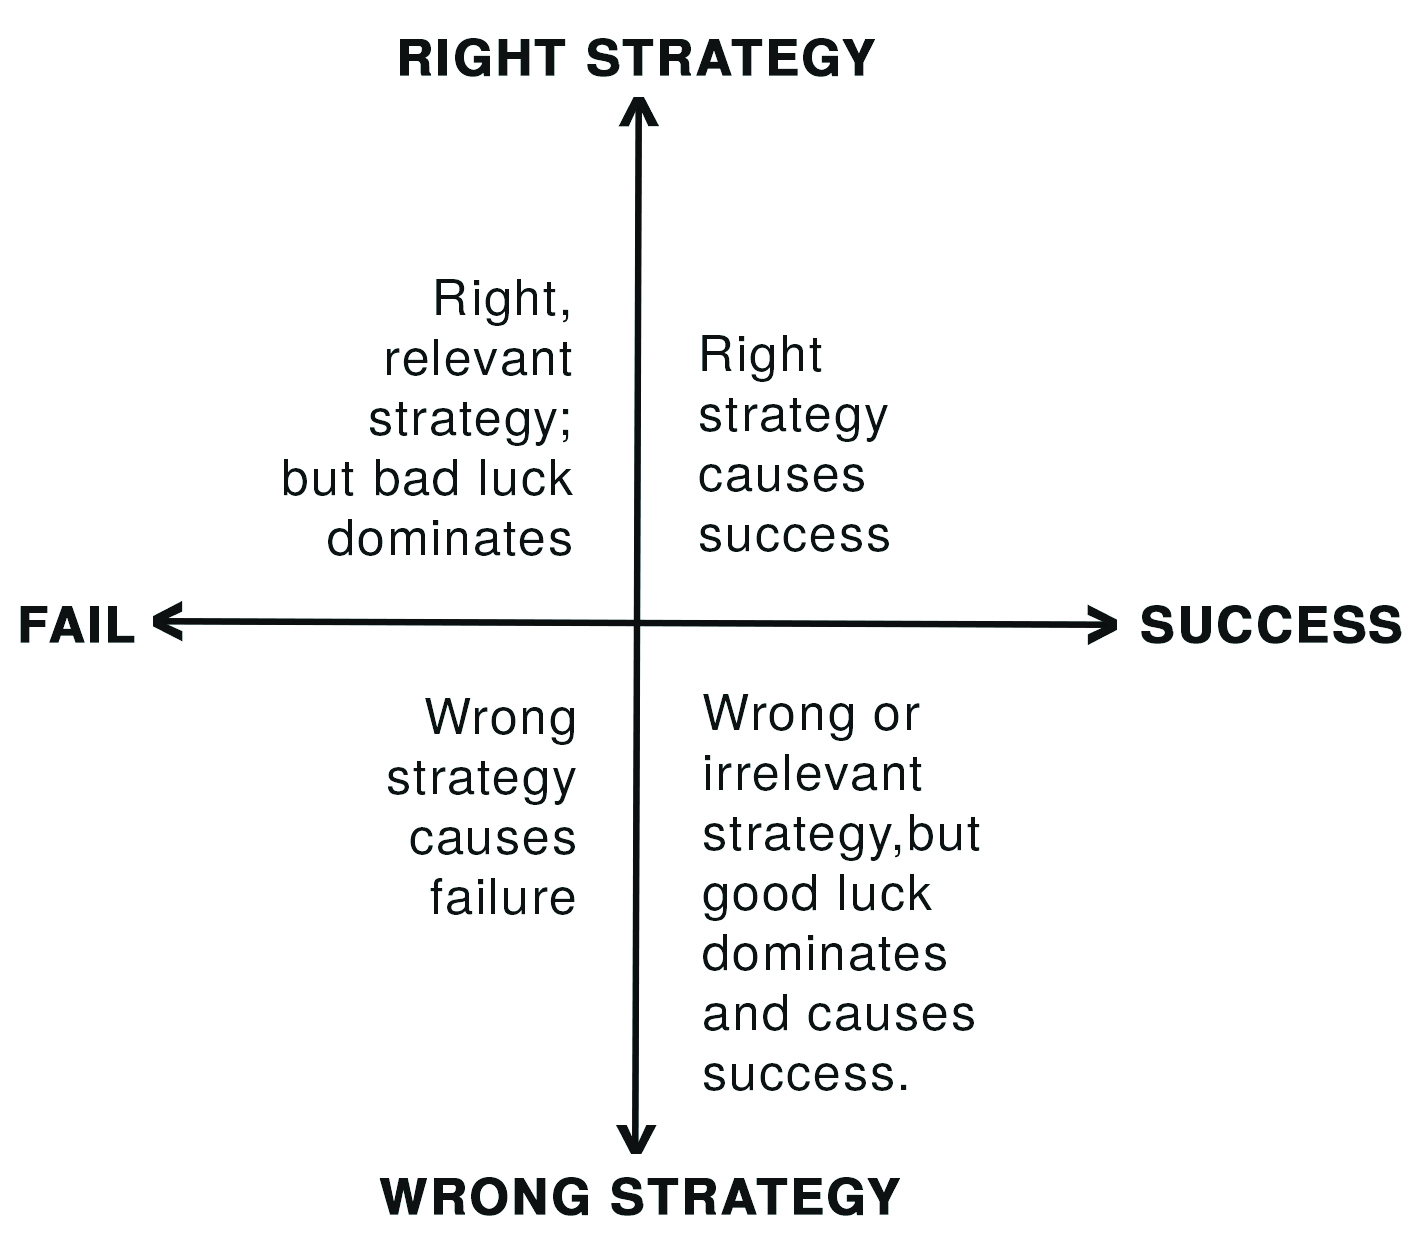
\includegraphics[width=0.70\textwidth]{./Images/Vuca-Cause-and-Effect}\end{center}
\caption{Cause-effect square in a VUCA world, and the role of luck.}
\label{figure:vuca-luck}
%\end{wrapfigure}
\end{figure}


Post-logical thinking, at its highest level, is seeing that the 27 years of imprisonment on Robben Island ahead of you (if you were Nelson Mandela)\index{Mandela, Nelson}  might be part of your becoming the statesman, capable 27 years later, of leading South Africa\index{South Africa} through an awe-inspiring transition. Seeing that you are a prisoner and a leader, without any contradiction between the two, and still being fully a prisoner and fully a leader.


Post-logical thought forms are all about grasping opposites, contradictions and paradoxes to create transformation. Like seeing sources of hope\index{hope} in our fears, in our enemies.


\section{28 post-logical thought forms}
\label{section:dtf-description} \index{thought forms (28)|(}


The 28 thought forms (see Otto Laske's\index{Laske, Otto} second volume\cite{laske-vol2} and \emph{Metathinking}\cite{shannon-metathinking} by Nick Shannon and Bruno Frischherz for full details)\index{Shannon, Nick}\index{Fischherz, Bruno} extend the binary logic of true-false into forms of thought to enable you to get ever better at grasping the nebulous, VUCA\index{VUCA} actuality you live in. The better you can use all these forms of thought and logical thinking, the closer your reality can match the subtleties of actuality. 


Once you are fully fluid in these forms of thought, you fully grasp that unceasing change is normal, not exceptional. There's always more to what you're looking at than you can see; contradiction, conflicts, oppositions, paradoxes, anomalies etc. are inherent, with no way of reducing them to binary logic. Everything is part of a bigger whole, connected to multiple different things, nothing is isolated or independent. And there is always potential for transformations that you cannot see or predict from where you are now because there are always more lenses, perspectives or input needed to fully grasp actuality than you are using.


When you look at the 28 thought forms in Table~\ref{table:28DTF}, you may recognise them all and think that you already use them all with a sufficiently high fluidity. Very few people really have the capacity to use all 28 thought forms with full fluidity when facing challenges. No matter how good you think you are, you can grow in mastery.


You can only learn how to use these 28 thought forms fluidly through dialogue with other people. I (Graham) initially tried mastering them solo and found that whilst I made good progress memorising the thought forms, a hundred times more fluidity developed through dialogue with others because they have different worldviews and use the thought forms differently.


These thought forms have been uncovered, over thousands of years, by all the world's different philosophers and religious thinkers. Otto Laske has distilled out this complete set of 28 thought forms, in four groups of seven each, summarised in Table~\ref{table:28DTF}.


\begin{description}
\item[Context:] these are thought forms that you use to fully grasp the static aspect of actuality. If you are only able to use context for forms, inner reality will be static, although perhaps extraordinarily complex.
\item[Process:] these are thought forms that you use to fully grasp opposites and simple changes or processes from one state to another. Process thought forms create an inner reality that far better represents the movement, change, and paradox of actuality.
\item[Relationship, or relatedness:] these thought forms go even further, giving you the capacity to grasp what is common, and the relationships between aspects of actuality that at first sight seem to have nothing to do with each other. They also give you the capacity to recognise relationship as an element of actuality in its own right, independent of any two specific things that are in relationship.
\item[Transformation:] the most advanced forms of thought, build on the foundation of context, process, and relationship thought forms. These transformational thought forms give you the capacity to rise to the biggest adaptive challenges.
\end{description}


\begin{table}[htbp]
        \small 
        \begin{tabular}{ L{0.02\textwidth} L{0.17\textwidth}  L{0.17\textwidth}  L{0.18\textwidth} L{0.20\textwidth}  }
                \toprule
                & \multicolumn{1}{c}{\textbf{Process}} &
                 \multicolumn{1}{c}{\textbf{Context}}  &
                  \multicolumn{1}{c}{\textbf{Relationship}}  &
                   \multicolumn{1}{c}{\textbf{Transformation}}   \\ 
                & \multicolumn{1}{c}{(P\textsubscript{i})} & \multicolumn{1}{c}{(C\textsubscript{i})} & \multicolumn{1}{c}{(R\textsubscript{i})} & \multicolumn{1}{c}{(T\textsubscript{i})}  \\
                \midrule
                 {\large 1} & Permanent movement &       The parts within a whole &  Limits of separation, existence of relatedness &  Limits of stability, harmony, durability. \\ \addlinespace[.5em]
                 {\large  2} & Including opposites &  The whole, its equilibrium &  Value of bringing into relationship &  Value of conflict for development \\ \addlinespace[.5em]
                 {\large 3} & Composed of interpenetrating opposites &  Structures, functions, layers of a system. &         Critique of neglecting relationships &  Value of developmental growth \\ \addlinespace[.5em]
                 {\large 4} & Patterns of interaction &         Natural hierarchy of layers of a whole &         Relatedness of different frames of reference &  Evaluative comparison of systems in transformation \\ \addlinespace[.5em]
                 {\large 5} & Knowledge always under construction, ne\-ver abso\-lute nor complete &  Stability of a system in its functioning &         Formal structure of relatedness &         Bringing multiple systems into balance with each other \\ \addlinespace[.5em]
                 {\large 6} & All always in motion; a form not thing. &         Frames of Reference, traditions, ideologies &  Patterns of interaction in relationships &  Open equilibrium systems in constant transformation \\ \addlinespace[.5em]
                {\large 7} & What is embedded in a bigger process. &  Multiplicity of contexts &  Constitutive relationships & Integration of multiple perspectives \\
                \bottomrule
        \end{tabular} 
        \caption[28 forms of post-logical thought]{28 forms of post-logical thought, based on Laske\cite{laske-vol2}.}
        \label{table:28DTF}
\end{table}




To get an idea of where you are, print out this table, and keep an eye on which forms of thought you are using during the course of a week or two.


These thought forms are devoid of content. Think of them as more like a modern kitchen full of all possible equipment, enabling you to create all kinds of dishes and tastes from common and unusual ingredients, because you can work at all scales, from molecular up, with all kinds of changes and transformations, and by bringing into relationship ingredients never connected before. (For example, Odyssey, the chef at Granny Dot’s\index{Granny!Dot’s}\index{South Africa!Granny Dot’s}, where Jack and Graham have written part of this, has just introduced us to pumpkin leaves with peanut butter. Surprisingly delicious!)


Cooking is assembling a puzzle in food. Your thinking is assembling reality as a puzzle out of different pieces from actuality. Each piece of the puzzle becomes an element of the content of your thinking, and by making meaning through your stories of the final assembled puzzle, you end up with your experience of reality.


If you use equipment unsuited to the shape and nature of the puzzle piece you are about to assemble, you will end up bending, squashing, or stretching it to force the pieces to fit together. So you end up with a distortion of the puzzle.


Similarly, if you use an unsuitable or clumsy thought form to grasp a piece of actuality and bring it into your awareness, you will distort it. But, because you have distorted it at first contact, you cannot realise that you have created a poor representation of actuality in the assembled puzzle that is your reality. 


In other words, whilst you believe you have grasped what is actually happening, you have not. You have created a distortion that you cannot see.


Sense-making\index{sense-making}  is the name we give to the process of assembling what you are aware of into a complete representation of actuality. If you have distorted this representation because you lack the necessary fluidity in the appropriate thought forms, the next stage of meaning making will be even more distorted. 


Rising to your adaptive challenges\index{challenge!adaptive}  becomes easier the more fluid you are in using all 28 thought forms. You become better at recognising clearly the meaning-making stories that run you, the big assumptions that you are subject to, and then creating the experiences you need for your stories to rewrite themselves.


The better you can do this, the more effectively you can lead yourself through life, and your organisation and staff to success.






\section{Process, movement thought forms}
\begin{quote}
To oppose something is to maintain it.\\
\raggedleft\textemdash Ursula K. Le Guin\index{Le Guin, Ursula K.} 
\end{quote}


This quote from Ursula K. Le Guin is, for me, a most thought-provoking quote. I have realised that some things I have done to try to oppose the causes of climate change are instead making it harder for us to get to a viable human society with an economy that works with, not against, nature's economy.


Consider, as you read this chapter, what these process thought forms can show you about how your actions are maintaining the very things you are trying to change. After all, one of the best ways to maintain something is to resist it!


To compare the first two sets of thought forms, process and static context, imagine you are about to hire someone. Is it the decision point that you focus on, and the gap in the organisation chart? Then you are using static context thought forms. 


Or is the decision point for this recruit simply one fleeting stage in a sequence moving towards an ever higher-performing workforce? And so no decision can ever be \emph{right}, but only just one step in a journey that began a long time ago, and will continue deep into the future? Then you are using process thought forms.


You may hire the best person to raise your team's overall performance. But immediately anything changes, for whatever reason, that may no longer be the best person to raise the performance. The team may change for external reasons, because its work changes, because someone else in the team changes, whatever. 


So process thinking makes clear that you can never hire the right person if you only hire for the job you need filling now. But if you hire people who bring skills you need now and can adapt themselves, can learn new skills, and can bond well with others, you will continue to have a good team as things change over time.


\paragraph{\textbf{P1: Permanent movement.}}
You are using this thought form when you are aware that everything is on a journey from past to future, changing all the way. You're using this thought form, when you are aware how the past is part of the present; and even the future is part of the present. 


For example, the more aware you are of how your thoughts about what might be in the future actually shape your choices and experiences in the present, the better you are using this thought form. 


Permanent movement, P1, also includes awareness that things are constantly changing into their opposite, or the complementary component of a complementary pair.\index{complementary pairs}  E.g., the bigger an organisation grows, the closer it gets to collapsing and shrinking as it outgrows the strength of the structures holding it up.
\paragraph{\textbf{P2: Including opposites.}}
This is where you shift\index{shift}  from \emph{either-or} into \emph{and} thinking. A classic example of this was developing the concept of servant leadership: the recognition that the leader is also there to serve their followers, in ways that enable the followers to deliver better results. Traditionally, people thought that it was the follower’s job alone to serve the leader. Applying P2 made it visible that each is serving the other. Similarly, managing your manager is an application of P2. 


Just as in a complementary pair, there's no victory of one over another here, rather it's just the inclusion of opposites to construct a greater whole.
\paragraph{\textbf{P3: Built of opposites.}}
This is the next stage, building on P1 and P2. This is a foundation of complementary pairs in quantum physics. Here, you go beyond merely including opposites into seeing how something is inherently constructed from opposites. For example, juggling is built up of the opposites of gravity\index{gravity} pulling down and the juggler's hand pushing up. An electron is inherently and irreducibly both particle and wave, even though classical physics\index{physics!classical}  cannot allow any entity that is simultaneously both. 


You, your organisation\index{organisation}, and society\index{society}  as a whole, works, has strength and stability because the whole is constructed from what we would normally see as opposites. If you try to fix yourself, or your organisation, by removing parts that you deem “bad”, you may wreck something that you value because everything is built of apparent contradictory opposites that are both required.
\paragraph{\textbf{P4: Patterns of motion and interaction.}}
P4 is about patterns of motion, where two or more distinct things have a pattern of motion relative to each other. For example, as the leader, you may get angry with a colleague, leading them to make a mistake in their work through nervousness, leading you to then recognise your role and apologise, or just getting even angrier with them. If this only happens once, all you need is P1. Usually, though, this is a pattern of behaviour that the two of you have got into. Each of you is in constant movement versus the other in a clear, distinct pattern. Just like the earth is in a pattern of motion around the Sun. 


P4 is the thought form you are using when you really understand what that pattern is and what causes it, as Newton\index{Newton, Isaac}  did when he thought that the force of gravity caused the Earth to rotate around the Sun, and as Einstein\index{Einstein, Albert}  did even better when he realised that there was no force of gravity, rather a closed circular pattern in curved spacetime where the earth and sun moved relative to each other without any force of gravity, but with an apparent interaction mediated by the curvature in the geometry of spacetime.\index{spacetime} 
\paragraph{\textbf{P5: Knowledge under construction.}}
You are using this thought form whenever you are able to see clearly how something that you know, is just knowledge that you have actively constructed, and because you've actively constructed it, it can never be complete and absolute actuality.\index{actuality}  It is always part of your internally constructed reality. 


The choices you make about what elements to add to your knowledge construct, and how, always have some practical shaping driver. You construct knowledge because of some practical use you want to put it to, and this use is a consequence of your meaning-making stories. Maybe you are just a collector of knowledge, like a stamp collector wanting to have enough of it to arrange in beautiful patterns and present to others; or, you want to use the knowledge to beat other people by exploiting a weakness.


The better you are able to use this thought form, the better you are able to recognise that what you have, until now, taken as an absolute; that that is the way the world is and has to be; is your personal construction determined by your practical needs emerging from your meaning\hyp{}making. 


This is especially true for any knowledge you have about yourself or any other person. That knowledge is always a very sparse representation of who that person actually is, and is something that you are constantly and continuously constructing and reconstructing. 


Similarly, once you see an organisation as a living being, you realise that you can never know it, rather you are constantly constructing the best approximate knowledge that you can. Disciplines like economics\index{economics}, or any social and physical sciences, are always a body of partial knowledge under constant construction.
\paragraph{\textbf{P6: Don’t concretise, a form not a thing.}}
Picasso\index{Picasso, Pablo}  got this right, when he said 
\begin{quote} 
If I paint a wild horse, you might not see the horse \ldots but surely you will see the wildness! 
\end{quote} 
He recognised that if all you do is think of a horse as a thing, you miss almost everything that differentiates a horse from an identical statue of a horse.


A horse is always in motion, not random motion, but motion within some form. If you think of yourself, or your organisation, or society and its economy as a whole, as a thing that you can understand in itself without movement, the ebb and flow of interaction, all you can grasp is a shadow frozen in time. Rather, it is not a thing, but a form, an entire collection of certain allowed motions, changes, processes, etc., that together give the form of a wild horse. One moment that form looks like a thing, the next moment it looks like another thing, or a process, or a relationship.


Whenever you are unable to see the form, but only a concretised “thing” instead, you miss 99.9\% of what you can do to lead change. Seeing yourself, or the legal structures to incorporate a business as a non-human legal person, as things you can only accept or reject, rather than forms that are always moving and changing, is one of our biggest barriers to creating an economy that works for you, for our planet, and for profit. Concretising what is actually a fluid flowing form into a thing is one of the cognitive weaknesses holding us back.
\paragraph{\textbf{P7: Embedded in bigger processes.}}
Expanding P6 to everything, you see that a whole is itself a form in constant flow, composed of ever more forms themselves in constant fluid flow. Everything is embedded in a larger flow and composed of entities in a smaller flow. You can only really use P7 after you have mastered, and can use fluidly, all the previous process thought forms.


So to understand anything happening in your life, you need to look at all the flows that you are embedded in. These might be processes that began in your childhood, a process of change and movement that has got you to where you are now. If you don't look at the entire sequence of changes, and choices, you will misunderstand what is happening to you now, and very likely choose poorly out of the options you have.


Even more, what happened to you in your childhood is a consequence of all the processes of your parents, and of all the other family members around you, from the moment they were born. Without having enough understanding of these even bigger processes, you are likely to misunderstand what is happening in your life now, and which option ahead of you is the wisest to choose.


Even more again, all of that is a consequence of the processes going back generations. Which is why many traditions around the world ask anyone taking a decision to look at the consequences of that decision over the next seven generations.


\emph{The economy, stupid} is a phrase coined by James Carville,\index{Carville, James} a US political consultant, in 1992, in response to a question. He clearly recognised in this response the importance of taking into account, for even the smallest of questions, the consequences of all the processes we are embedded in, up to the very largest.




\section{Context, structure thought forms}
The next seven thought forms are static structures and constructions. If you are about to hire somebody, and look at their university's ranking in the current tables, the courses they studied and the results they got, you are using context thought forms.


Just as the process thought forms do not deal with context and structure, these thought forms do not deal with processes of movement and change, nor with the inclusion of opposites to create something new that is different to just the opposite put together. Nothing changes in any of these thought forms.
\paragraph{\textbf{C1: Parts within a whole.}}
The better you can use this thought form, the better you can understand any part of a whole, because you have grasped the context that the whole gives to the part. For example, you are a part of a bigger whole, a family, or a group of friends. How is who you are shaped by being part of that family, or group of friends? How do you in turn shape them?


Whenever you only think of yourself or anything else in isolation, you are quite likely to misunderstand what is actually happening by neglecting the shaping influence of being part of a bigger whole.


Becoming aware of all the different parts that make up the whole is vital in creating a better reality out of actuality. For example, recognising that I am built up of many different parts helped me see my digestion as one part, my blood and blood vessels as another part, and my brain a third part that all need to be taken into account to understand my depression. So whenever something is happening, and you suspect that you haven't grasped enough, always look for additional parts that you may not be looking at, and the larger context that you're not yet seen clearly.
\paragraph{\textbf{C2: The whole.}}
If you're looking at the whole as a whole, where each individual part is more background, you are using this thought form. You are using this thought form, when you recognise that the team as it \emph{is}, is composed of all the people in it, so introducing one new person to the team might lead to a completely new team dynamic, not just a slight modification.


When you ask yourself whether your team is a big enough whole, or rather you should look at the organisation as the relevant big enough whole, you're using this thought form. 


The emphasis here is really on zooming out until you have identified the biggest whole necessary to grasp what is going on, and an understanding of how the essence of that whole emerges.


\paragraph{\textbf{C3: Structures, functions, layers of a system.}}
Sometimes the whole might just be a random jumble of parts, as if you had taken a box with all the pieces of the car kit and looked at the contents as a whole. Yes, it is a whole car kit, but it is far from being a whole kit car.


A whole car has all the same pieces, but arranged in a hierarchy of parts. You have a hierarchy from the bottom to the top, beginning with the tyres and ending with the roof; you have a hierarchy from front to back, beginning with the headlights and ending with the taillights; and you have a hierarchy of function, such as the brake pedal activating the servo motors activating the hydraulics activating the brake pistons which squeeze the pads against the discs leading the tyres to slow down.


\paragraph{\textbf{C4: Natural hierarchy within a whole.}}
Going one obvious step further from C3, you realise that any functioning whole has a natural hierarchy of layers and functions. Even if you tipped your box of car pieces onto the floor of your garage in a pile, gravity would impose a natural hierarchy. Any piece that was not strong enough to support the weight of the pieces above it would deform until what was left was strong enough.


The better you understand the natural, essential, hierarchical arrangement of parts within a whole, the better you can figure out what is going on, and what to do about it. For example, without understanding the natural and necessary hierarchies within organisations, some misinterpret the emerging approaches to dynamic organisation design and governance like Holacracy\index{Holacracy}  and sociocracy\index{Sociocracy} as hierarchy free. They can still be hierarchical, just the hierarchy allows it to be context-dependent and locally adaptable, rather than identical in all contexts and requiring approval from above to change. 


Such essential hierarchies are hierarchies of complexity, rather than hierarchies of person. For example, if I go to an excellent doctor, we both recognise that there are two hierarchies simultaneously present: I am at the top of the hierarchy of knowledge of my experience of my illness, and the doctor must accept that to be a good doctor. They are (I hope) superior to me in understanding health and illness, and the ability to see a successful treatment in the data of my symptoms. Blindness to either of those essential hierarchies will lead to a substandard or harmful outcome. As the permanent damage one doctor caused to my (Graham’s) left ear is testimony to.
\paragraph{\textbf{C5: Stability of a system.}}
One question that led me to the content of this book illustrates C5: 
\begin{quote} 
what is keeping our dysfunctional system stable in its dysfunctionality? 
\end{quote} 
because I recognised that our economic and business systems have proven enormously difficult to change, despite decades of intense effort by very many people. 


By asking what keeps the whole system stable, even though it's widely recognised as dysfunctional, enabled me to understand why more regulation, more effort on values-based leadership, and more corporate codes of conduct were at best going to make marginal differences. We need to pull out the pins of shareholder primacy that keep the system stable.


Even worse, by fighting against the system with those pins in place, we might even maintain the system. Picture a tug-of-war; the very fact that you have two teams pulling against each other is what keeps the rope off the ground and stiff. Or, consider the punitive justice system used in most countries. That system is kept stable because all the opposing elements reinforce each other. No part of the system can change unless the whole system changes. Changing the whole system is what South Africa did, e.g. via the Truth and Reconciliation Commission, which prevented a countercoup.


Until you are viewing a system sufficiently holistically, with an understanding of what keeps that whole as it is, you have little chance of generating any change to the system. C2 and C1 are two thought forms used in the ground pattern of Chapter~\ref{chapter:who-am-i-meaning} to understand who you are, and grow into who you can be, by triggering the very instabilities needed for who you are to become a process of growth, not a static identity.


\paragraph{\textbf{C6: Frames of reference.}}
This is one of my favourites, and you have already read these words many times throughout this book. Every single time you make a choice, that choice is based on an ordering of options determined by the C6 frame of reference you are comparing each option against.


A common misunderstanding of Darwin's survival of the fittest is that it means survival of the strongest. Any business leader using that as their frame of reference will build an organisation and strategy around overpowering enemies with strength.


However, a business leader who understands evolution recognises that the frame of reference Darwin\index{Darwin, Charles}  used is that \emph{whoever is the best fit to their particular business context, and is most able to adapt as that business context changes, is most likely to survive}. Using this, \index{frames of reference} they will choose, depending on the bigger picture (C2), to collaborate, compete, or some mixture of the two (P2, and perhaps P3 in some cases). By using this different frame of reference, from exactly the same actuality, they follow a different strategy leading to different choices.


Until you look at the options you are choosing between, and the frame of reference you are using to evaluate those choices as one complementary pair\index{complementary pairs}, you have an insufficient grasp of what is happening. This is especially true whenever you are judging yourself, anyone else, or any situation. If you fail to take into account the frame of reference that is always part of any judgement, you are taking a blind step, which in the worst case may cause irreparable harm to you and your business.


The game of paper, stone, and scissors is a perfect example; which beats which depends on the Frame of Reference, rather than being an absolute property of the paper, stone or pair of scissors.
\paragraph{\textbf{C7: Multiplicity of contexts.}}
As with P7, C7 depends on all the other context thought forms and takes them onto the largest possible stage. C7 is when you are easily able to look at multiple contexts to see and work with more of actuality. These different contexts may well have nothing to do with each other or may also, from another perspective, be different parts of an even larger context.


For example, you may have a direct report that is delivering substandard results. You recognise that you need to look at them in the context of the team they are part of and the organisation that that team is part of. So you realise that part of their performance problem lies in how the roles are split between themself and their colleagues, and so you modify the role definitions and accountabilities.


You also realise another distinct context is their family life, even bigger, all the team members’ family lives, that each one arrives at work still part of each of their family contexts. Any worries or joys in their family contexts are shaping what they do at work.


Then you think how each of them is carrying their own personal context of internal meaning-making stories that tell them what to do. Without fully understanding what this context is telling them to do, you will be missing some vital intervention needed to address the performance issue.


Throughout all these context thought forms, the more fluidity you have in each and all of them, the better grasp you can have of what you are actually dealing with in any instant.






\section{Relationship/relatedness thought forms}
These thought forms span all kinds of relationships between all kinds of entities, not just human relationships between people. 


\paragraph{\textbf{R1: Limits of separation.}}
You are using this thought form when you are aware that two things that might each appear to be unique and completely distinct, are actually connected and have common ground. Even more, if you actively say that two things are connected, even though everybody typically thinks they are separate, and then look for the common ground, you are using this thought form.


Most isms originate in an inability to use this thought form. Racism\index{racism} lies in an inability to see that someone of a different skin colour shares as much or more common ground with, than difference to, every other human being. 


Businesses collapse, and nations collapse, when their leaders lack sufficient fluidity in R1 to recognise the limits of separation and fail to stand sufficiently in the common ground that connects individual businesses and nations. 


No single nation can thrive if the polluting CO\textsubscript{2} from all nations changes the atmosphere's insulating properties to the point where the global economy collapses, because much of the earth ceases to be viable for human life. An inability to use R1 is a root cause of many of today's intractable problems. 
\paragraph{\textbf{R2: Value of bringing into relationship.}}
You are using this thought form when you see clearly how it becomes valuable to connect two things that are separate. For example, the standard limited company separates, with a very hard boundary, investors from all other stakeholders.\index{stakeholders} Using R1, you see that the common ground of all the stakeholders lies in all of them being stakeholders in the same business, with a stake in the business’s success.


R2 then shows you how changing how businesses are legally incorporated, to bring the stakeholders into a relationship with each other where all are part of steering the company into the future, and sharing the wealth generated, has enormous value\index{value}. You eliminate many losses from the artificial and costly fights between them, and you bring into business decision-making, for the benefit of the whole business, information that only one stakeholder category may have. Enter the FairShares Commons.


R2 plays a role in developing yourself and enabling your meaning-making stories to rewrite themselves, by enabling you to see the value in the relationship between different aspects of your self that you have, up until now, believed were distinct.


This thought form is vital for economists\index{economists}  to develop a real understanding of how an economy actually works. Without a deep understanding of the value created when individual and collective meaning making, and social processes and economic choices, are brought into relationship with each other, no broad theory of an economy can be developed.
\paragraph{\textbf{R3: Critique of neglecting relationships.}}
You have already seen examples of this thought form in the above paragraphs, where I criticised the fact that many academics and leaders in economics\index{economics}  and business fail to see clearly how all the different stakeholders in every business, and of course the economy as a whole, have to do what they do because of the relationships. 


Whenever you recognise that actuality is far more deeply interconnected than the reality\index{reality}  you are able to perceive, and where you refuse to accept that a disconnected reality is enough to get a good enough idea of everything important that is actually happening, you are using this thought form. 


When you point out the complexity that is missing by ignoring its relationships, and the absolute necessity of including that complexity to be able to decide what to do next, you are using R3.
\paragraph{\textbf{R4: Relatedness of different frames of reference.}}
In C6 you are thinking about a frame of reference; how an awareness of the frame of reference and the judgement made against the frame of reference is equally necessary to understand your judgements and choices.


Using R4 you see clearly how different frames of reference are related to each other. These might be different frames of reference inside yourself, or differences in the frames of reference you and your colleagues are using when faced with the same choice.


Imagine you are part of a startup leadership team needing to take a decision on whether to bring in venture capital (VC) money, borrow from the bank, or bootstrap on cashflow. You might all use C6 to give your choice, with the reasons why you think that is the best decision and the frame of reference you use to define best. Each person may well have a different choice, set of reasons, and frame of reference.


Now you start looking at what the relationship is between each frame of reference, and for the common ground uniting all the frames of reference.\index{frames of reference}  By doing that, you may end up with a larger frame of reference that gives you one single choice which everybody agrees is the best.


That will be a very different discussion to the one many leadership teams usually have: just arguing until one option is left standing, without ever understanding the frame of reference each person is using in that argument. 


Better leadership teams surface first each frame of reference and argue about those until they find one to use.


The even better leadership teams uncover the hidden relationships between all the frames of reference, integrate them into a bigger inclusive frame of reference, and take a decision on the common ground.


You are also using this thought form when you are able to recognise the relationship(s) between different individuals' value systems, and between different cultural value systems, even though the actions taken to express the value systems may be completely different. For example, in some countries it is polite to blow your nose (e.g., UK, Germany, US), and in other countries it is polite to sniff (e.g., Japan). The two conventions are related by common values: respect for other people, harmony, and social cohesion.
\paragraph{\textbf{R5: Formal structure of relatedness.}}
The quote from Ursula K. Le Guin\index{Le Guin, Ursula K.}  at the start of the Process section points at this. There is an underlying structure in the oppositional relationship between those supporting a system and those fighting against the system. For example, consider the battles between a trade union and a company. There is a formal structure that relates them, in that both exist because of the apartheid-like way companies  incorporate, denying stakeholder relatedness. 


Neither the union nor the company can achieve their objectives because they are trapped in a \emph{relationship} that lacks those objectives.


In many cases the formal structure of relationship maintains the status quo, even though huge effort is put into the fight against the status quo. The way forwards is to recognise the formal structure of the relationship and decide to step beyond that and invent a new structure. This is what the FairShares Commons\index{FairShares Commons}  does for the relationship between stakeholders, and between different kinds of capital.


The structure of a relationship may be so much part of the background, that it becomes invisible, or worse, unquestionable. Much like fish in water do not even see the water giving structure to the relationships between all purely water-based lifeforms. Any that were able to consciously recognise and question water as the only structural basis for the common ground of all aquatic life might figure out how to become flying fish.
\paragraph{\textbf{R6: Patterns of interaction in relationships.}}
This thought form is what you use when you’ve used all the earlier relationship thought forms, and grasped the existence of patterns due to the relationship in how entities interact.


You can begin finding ways of influencing without direct control if you are able to tap into these patterns of interaction.


The pattern of interaction might be one of opposition, it might be one of collaboration, or a mix of the two. The big difference between this thought form and P4 is that here your focus is primarily on the relationship, whereas in P4 you are blind to the relationship and only looking at the pattern of interaction. So those who are only fluid in P4 find it far more difficult to subtly influence what is happening around them, and may only be able to make progress by using power over others.
\paragraph{\textbf{R7: Constitutive relationships.}}
Many relationships are old. The relationship existed long before any of the individual elements even existed; the relationship shaped, or even created, the elements, rather than that the elements created the relationship only after coming together.


For example, a marketplace has pre-existing relationships going back many thousands of years, long before any specific buyer walked up to a specific seller. This pre-existing relationship shapes what the buyer and seller each do.


In apartheid South Africa,\index{South Africa!apartheid} the relationship throughout the entire lifetime of a specific white and a specific black was predefined long before birth. 


The relationship shaped the life experiences of a black baby and a white baby born at exactly the same time in the same hospital. When they meet for the first time, perhaps at 40 years old, they are already in a pre-existing relationship. 


Even if they first meet at 70, standing next to each other in an enormous queue of people snaking backwards and forwards waiting to cast their vote in the very first election in post-apartheid South Africa,\index{South Africa}  that pre-existing relationship has shaped who they are and what they do.


Recognising the pre-existing independent relationship enables them to interact from a place of compassion of how the pre-existing relationship has caused what they experienced, instead of directly blaming as if each person had complete freedom to develop the relationship from scratch.


If you are married, you and your spouse entered into a pre-existing relationship going back millennia that has shaped how each of you show up together. Similarly when you join a hierarchical organisation.


This is why it is so hard for a couple to change themselves and their behaviour within the relationship; why it is so hard to restructure from a hierarchy to a sociocracy; the generations-old pre-existing relationship shapes what you do.




\section{Transformation thought forms}
Now we get to the transformational thought forms, the seven most powerful ones to address our global challenges. But, until we are sufficiently fluid in context, process, and relationship, we can't become fluid in the seven transformation thought forms.


The Dunning-Kruger effect\index{Dunning-Kruger effect}  (Section~\ref{section:dunning-kruger}) applies, in that many people imagine that they can use these thought forms. While cognitively they understand what is written, they lack the fluidity they need in all the thought forms to recognise what these thought forms really entail. They are not good enough to know how weak they are, and so imagine that they are good, or at least average.
\paragraph{\textbf{T1: Limits of stability.}}
There is no stability across all time\index{time}  and space\index{space}, let alone anything smaller. You are not stable, your relationships with other people are not stable, nor are the companies that you work in stable.


When you recognise that there are limits to stability, you can begin to work with them. You can begin to accept that a relationship may break down because there is an inherent limit to the stability of that relationship over time or under external pressures. Then, you can more easily recognise the difference between not having done enough versus the impossibility of maintaining the stability of that particular relationship.


The more aware you are of the limits of stability, accurately and in detail, the better you can identify what to do to maintain the stability, if that is important; the better you can accept disharmony as inherent, without taking it personally; and the better you can understand why the system may be so easy to knock into instability. The more fluid you are in using this thought form, the less personally you take disharmony or changes in your life, and the better you can begin to tap into instability.


\paragraph{\textbf{T2: Developmental value of conflict.}}
This is a tough one for those of you who have a need for harmony in your nature or meaning-making stories. The developmental value of conflict\index{conflict}  is a thought form at the heart of this book. You grow as a human being through conflict, and your business grows through conflict.


You are using this thought form if you have a conflict and react with joy because you know that the simple existence of conflict means that you have potential to develop yourself, and likely the other person has potential to develop themselves.


You are using this thought form when, instead of your pain leading you to manage or resolve conflict quickly, you stay with the conflict, or even broaden it to include even more elements. You do that to be able to identify all the developmental golden nuggets buried in the conflict.


Living organisations\index{organisation}  today that really know how to mine and refine conflict are the ones most capable of transforming themselves and their collective meaning making, so that they thrive long-term because they remain a superb fit to their business drivers, no matter how fast those business drivers are changing.
\paragraph{\textbf{T3: Value of developmental growth.}}
T3 goes even beyond recognising that conflict can have huge value, into recognising the value of development. All the chapters in this part are about the value that you can get by developing your stage of meaning-making stories\index{meaning-making stories}, and your cognitive capacity to use the 28 thought forms fluidly. The other parts of this book are about the value of the same kind of development of our business systems and our economy and society as a whole.


You are using this thought form only when you go beyond simply saying that there is value in development, into actually describing what that value is; describing what needs to be done to trigger and guide development to access that value.


Business leaders who are insufficiently fluid in this thought form have difficulty keeping all the existing operations running unchanged, and delivering the cash needed to keep the business alive, whilst simultaneously leading the transformation needed for the business to adapt to its changing drivers.


Business leaders who are really good at this recognise when the old divisions between structures, processes etc., are no longer fit for purpose, and the potential in integrating parts of the system that have previously always been separate, in ways that lead to higher stages of complexity. For example, the shift\index{shift} from running a business selling books to running a platform that sells everything, as Jeff Bezos did.


\paragraph{\textbf{T4: Evaluative comparison of systems in transformation.}}
The final four thought forms are the most challenging to even begin using, let alone use fluidly; yet they are essential to transform our society and its economy to one that works for everyone, for our environment that we all depend on for life, and for the profit essential for our economy to function.


You are using this thought form, when you compare our current business system with the kind of business system that will emerge if every single company was incorporated as a FairShares Commons,\index{FairShares Commons}  and measure them against multiple frames of reference\index{frames of reference}  to judge which system is better for what outcome.


You are using this thought form when you fully grasp how each system can contribute helpfully or harmfully to dealing with the challenges we face. If we have a system including a tax on carbon pollution, how will that be a better or worse system than a very different one based on legislation mandating a zero-carbon economy powered by hydrogen and renewable electricity? What other structures and processes are relevant; how does each compare to the other; and which frames of reference\index{frames of reference} have relevance in order to evaluate them?


I was using this thought form when I looked at how freedom\index{freedom}  as an institution\index{institutions} has transformed individual satisfaction and development, then took that as a guiding template for how we might transform business systems composed of very large numbers of individual non-human legal persons.


\paragraph{\textbf{T5: Bringing multiple systems into balance with each other.}}
Thought form T1 introduces you to the limits of stability that trigger transformation of systems. Far more challenging is to bring systems, and even multiple systems, together and into balance, using T5.


You are only using this thought form if you've really grasped in sufficient detail, complexity, and holistically, what each system entails, and what it really means to bring the systems into balance. Given that living systems are, to a high degree, inherently nebulous and unknowable, if you are more aware of what you don't know than what you do know, you may be beginning to use this thought form.


You are using this thought form well when you're very aware of where each system is coming from, the contexts, including the dominant meaning-making stories that were concretising each system. And when you’re very aware of just what needs to be preserved of each system’s functionality while you are bringing them into balance with each other, even as you recognise that that functionality may be toxic for the final balanced system.


You are using this thought form well when you're using multiple frames of reference\index{frames of reference}  to evaluate your choices against, and meta-frames of reference to evaluate the frames of reference in order to decide which ones are helpful and which ones are harmful.
\paragraph{\textbf{T6: Open systems in constant transformation.}}
The previous transformation thought forms are blind to how all systems are open in some way, inseparably part of bigger systems, and in constant transformation. The earth is far from being a closed system. There is a constant flow of energy into the earth from the sun, and up until a few decades ago a constant equal cooling radiation of energy from the earth out into space. The growing carbon dioxide pollution in the atmosphere is upsetting this delicate open system balance by reducing the outflow of energy. Like a car with a radiator blocked with dirt, the engine is starting to overheat.


So when you're busy working on transforming the system, you need to use this thought form to fully grasp what it is that you're working with and what the consequences might be of any change. If you think that the system is closed, and you neglect to take into account what needs to be done outside the system with inflow and outflow, you will fail. On the other hand, if you can take into account how the system is anyway in constant transformation, and nudge it along more quickly where that helps, and slow down where it doesn't, you can begin to work magic.


You are using this thought form when you grasp both the opportunities and the risks in opening the system more, or in new areas, or closing the system where it is currently open. Linked to this is understanding what the necessary self-identity is of the system and what maintains it, and therefore that needs to be preserved as you work on the system.


You are using this system when you fully grasp how its openness and inherent transformations might affect you and your business, and therefore what strategy you need, and how you execute that strategy with excellence. All the while tempering what you do knowing that everything is inherently nebulous and your knowledge is under construction (P5).
\paragraph{\textbf{T7: Integration of multiple perspectives.}}
This is the most challenging thought form of all for anyone to even begin using, let alone to reach high fluidity in using unaided. 


This thought form lies at the heart of Cubism\index{Cubism}, relativity,\index{relativity}  and quantum physics.\index{physics!quantum}  Few people even begin developing the capacity to use this thought form, let alone use it fluidly. Fluidity in T7 is essential for anyone playing a pivotal role in guiding our social systems and institutions, especially economic and political, into a future that can work for the many by addressing all our global challenges.


Insufficient fluidity in this thought form is what leads experts to try to use their formalism even harder, not realising that the very attempt to use formalistic approaches is the problem.


You are using this thought form when you both use and dispense with using formalism in addressing the challenges. You are using this thought form when you use multiple, often contradictory, perspectives to understand what is happening. This is a challenge for people who have self-authored an integrity with one specific perspective on what integrity is, where that very integrity prevents them from seeing clearly the full complexity of what is going on.


How hard this is, is apparent when budding physicists\index{physicists}  are learning quantum physics. Quantum physics\index{physics!quantum} works because it is filled with multiple conflicting perspectives. To truly grasp what it means for an electron to be both a particle and a wave, to be at a point in time and spread out, is challenging even for the most advanced physicists. So early on, budding physicists learn that the equations really work, and how to use them to predict correctly how to build a smartphone, even when they haven't yet understood how these conflicting perspectives can ever come together to yield equations that work.


You are using this thought form well when the difference between actuality\index{actuality}  and the model you construct to represent it\textemdash reality\textemdash is immediately and always apparent to you. When you grasp precisely when not to trust your own experienced reality,\index{reality}  but look for other complementary realities that might shed more clarity on what actually is.


This is where you realise just how deeply connected everything is. That trying to separate structures, processes, individual and collective meaning-making, etc., and deal with each alone can never really work.






\section{Executing with excellence}
You may enjoy wrestling with these thought forms and developing your fluidity for the sheer pleasure of mastery. After all, mastery is one of the topmost human needs, and meeting that need is a source of joy for almost all of us.


I hope that most of you will go beyond intellectual mastery of the thought forms and into practical mastery by applying them in business. To deal with our global challenges and build a better world we need many more people who are able to do their work with excellence because they are highly fluid in all the thought forms.


Even more so because these thought forms are at their most powerful when used in dialogue with others; and you can only develop real mastery through dialogue with others. You need their use of a thought form before you can see clearly what is missing in yours.


Keep going, even if you cannot see where you are going, think you are making no progress towards any of your goals, and the effort of trying is unbearable.


I (Graham) used to row at school and university. As an oarsman I learnt to give all I had to reach a goal that I could not see until after I had reached it. I learnt to row until every muscle was in exhausted agony; and then just keep going, with little clarity on just how much further it was. (If you’ve not seen rowing, or rowed yourself, only the cox looks forward, the rest face backward.) Perhaps that helps me keep going now, even though I cannot see the finish line.
\index{thought forms (28)|)}